\documentclass{article} \usepackage[utf8]{inputenc}
\usepackage[english]{babel} \usepackage{hyperref}
\usepackage{graphicx}

\title{WV -- interim report} \author{Ward Schodts \& Xavier Goas
Aguililla} \date{31 March 2015}


\begin{document}
\maketitle

\section{A few practical issues}
\paragraph{LooCi and Contiki.} The initial intention was to
investigate energy measurements for LooCi components. Due to several
problems with over-the-air-deployment we decided to simplify our
approach a bit. We are now using pure Contiki on the Zigduino motes.

\paragraph{Output of the Matlab script.} The results of the power
measurements done with the oscilloscope all return negative units of
work. We assume that this has to do either with flow of current inside
the measurement setup or with the Matlab scripte we use. We interpret
these measurements as unsigned units.

\section{Interim results}
\subsection{Antenna}
\paragraph{Energy/byte.} We used the data provided at
\url{http://people.cs.kuleuven.be/~wilfried.daniels/energy/results3.html}
to roughly derive the energy cost per byte:

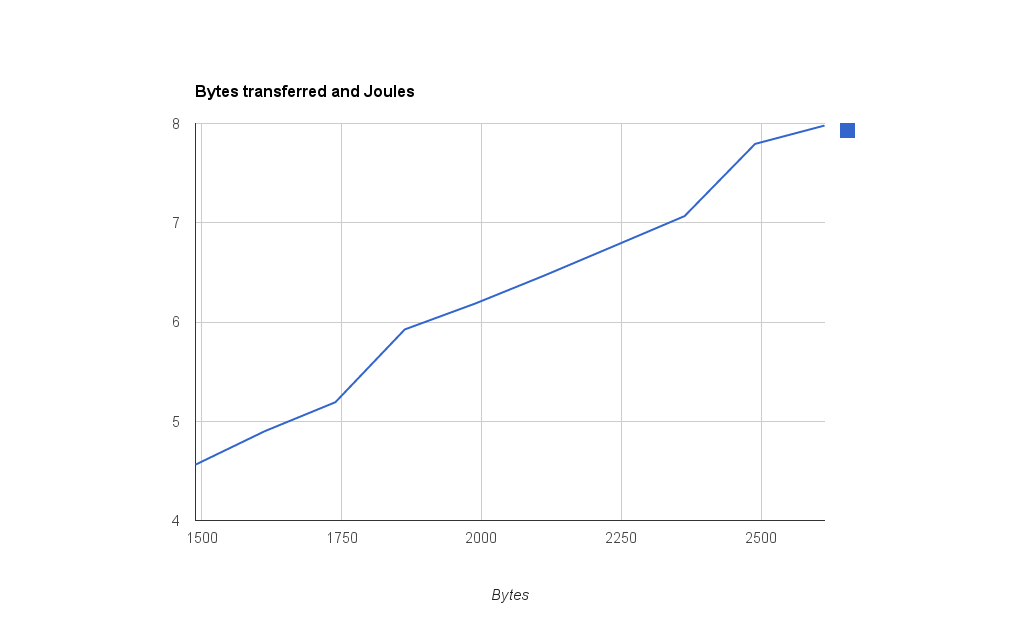
\includegraphics[width=\linewidth]{graph.png}

We obtained an average cost of $3.06399592 mJ/byte.$ by
extrapolating the data. Note that this represents the cost of
receiving a byte - we wonder if the cost of sending a byte will be
different?

\paragraph{Base level energy consumption.} Next, we also wanted to
know the base power usage when the mote is listening in low-power mode
and when the antenna is fully switched off.

To measure this, we wrote two `idle' components, the first with
low-power listening using ContikiMAC activated (as is default), the
second with the antenna and MAC fully switched off, and measured their
power consumption. The measurements performed on the second component
can be considered representative for the base power consumption of the
OS itself without networking functionality enabled. Subtracting these
results from the measurements on the first component gives a rough
idea of how much power low-power listening consumes.

\paragraph{Energy when idle.}
We got about the same energy usage as during the RAM test when we
wrote nothing:

\begin{verbatim}
-74.7316
-74.7610
-74.7003
-74.6391
-74.4582
-74.6195
-74.6579
-74.4509
-74.6454
-74.7656
-74.5681
-74.8548
-74.6121
-74.7943
-74.8279
-74.8777
-74.6717
-74.9203
\end{verbatim}


\paragraph{Energy when listening.}
During the listening test we got the following results:

\begin{verbatim}
-114.8897
-114.8994
-114.8356
-115.1350
-115.1103
-114.9205
-115.2339
-115.2512
-115.1336
-115.2102
-115.0942
-115.0485
-115.2242
-115.2833
-115.1356
-115.3479
-115.2736
-115.0013
\end{verbatim}

\subsection{Flash}
As discussed with Klaas, we will only research this option when we
have time. But it probably won't have any advantages: It most
certainly will cost more to write to flash and if you can use half of
the flash memory you only have 8 times more space to store data than
if you write to RAM (assuming you also use only half the RAM).

\subsection{RAM}

We wrote a component which repeatedly writes about 800kB of null bytes
to RAM. Between the repetition the mote does nothing and is idle. We
used the oscilloscope to measure a certain interval en we got the
following results:

\begin{verbatim}
-71.4368
-232.0165
-71.4722
-231.9092
-71.4422
-231.8196
-71.5196
-231.8710
-71.5787
-231.8401
-71.5961
-232.0866
-71.4173
-232.1306
-71.5185
-231.8660
-71.4893
-231.7818
-71.4970
\end{verbatim}

Energy when idle: $\pm 71 mJ$\\
Energy when writing: $\pm 231 mJ$
Energy for writing 1 byte: $ \frac{231-71 mJ}{8*1000*100} \approx 0 mJ$

We see that in fact writing a byte to RAM consumes almost no
energy, so that's definitely an interesting path to follow. But there's
an important question here. We didn't explicitly turn the radio off,
but the energy usage stayed the same between the writing intervals as
when the antenna is fully off. We're at a bit of a loss as what the
cause may be ...

\section{Conclusion}

All in all, we've made progress on some fronts. Accumulating data in RAM seems to be so cheap it would be a shame not to abuse it. Sending data on the other hand seems to be very expensive. The main problem is now twofold: how to measure power consumption for a given piece of component code, and how does the 'compute' part of the equation come into play? 

\section{Questions}
\begin{itemize}
\item Are our measurements reasonable and correct?
\item How to measure the CPU usage as described before?
\item How to estimate power consumption `at a glance'? (We're working on this)
\end{itemize}
\end{document}
